%!TEX root = ../../main.tex

\subsection{Evaluation of Event Clustering}
\label{sec:clustering}
\label{collection:sec:eval}
Since our event clustering approach is unlikely to be perfect and affects the number of events in our relevance judgements, an evaluation of its effectiveness is important.
Rather than directly evaluate the results of our clustering approach (i.e. similar to the evaluation of relevant tweets for a cluster), which would have made it difficult to measure any improvements in clustering quality, we wanted to gather relevance judgements which could be used to both measure and improve cluster quality.
\cite{Amigo:2009:CEC:1555682.1555686} define a number of constraints which need to be met in order for different aspects of cluster quality to be measured.
They compared a number of metrics and found only the BCubed metric~\citep{Bagga:1998:ECC:980845.980859} satisfied all of their constrains.
The BCubed metric measures the precision and recall associated with individual items in a distribution, with Recall representing how many items from the same category appear in the target's cluster, and Precision representing how many items in the cluster belong to the same category~\citep{Amigo:2009:CEC:1555682.1555686}. Since BCubed averages are calculated over items rather than clusters, this means that we can gather relevance judgements for a subset of the items, rather than the full 796, whilst still being able to accurately estimate the overall quality and choose the best parameters. Additionally, this means that it is not necessary to apply any weighting due to cluster or category size~\citep{Amigo:2009:CEC:1555682.1555686}.

\begin{figure}[h]
	{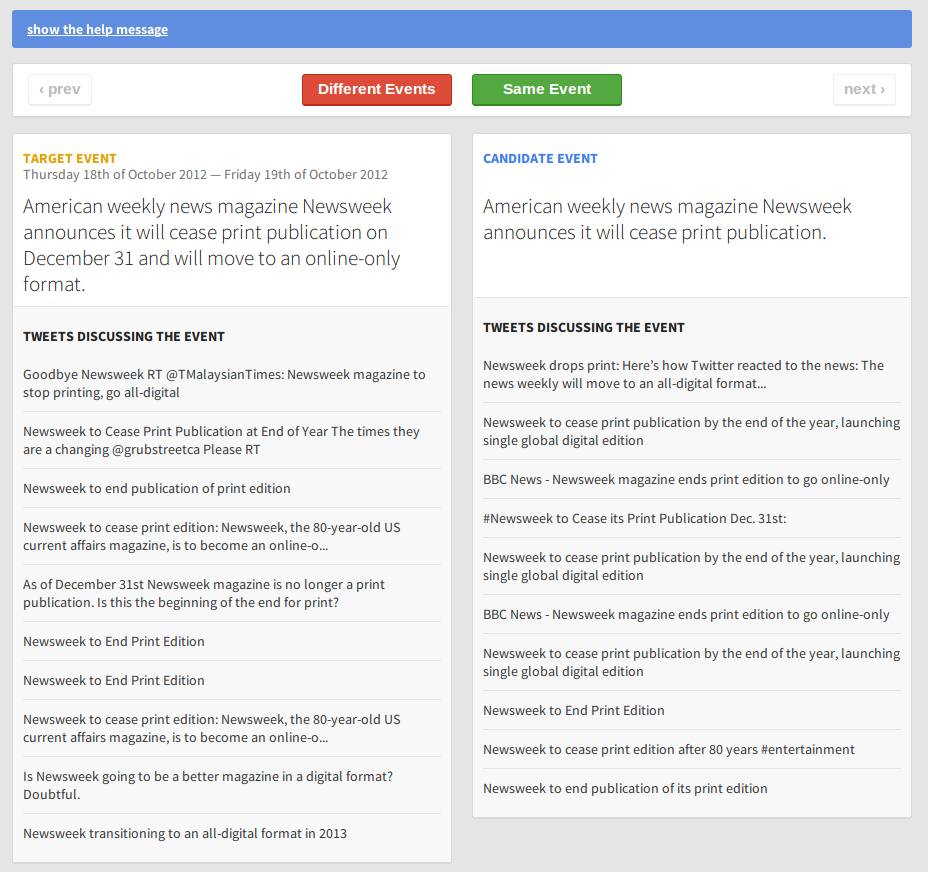
\includegraphics[width=\textwidth]{./Chapters/Collection/images/cluster_eval}}
	\caption{A screenshot of the cluster quality evaluation interface used by Mechanical Turk workers.}
	\label{fig:one}
\end{figure}

We took a random sample of 100 items (12.5\% of the total), which we refer to as \emph{targets}.
For each target, we identified 790 items which had centroid times (i.e. the average time of all the tweets in the item) within a 24 hour window (i.e. 12 hours either side of the target).
We call these items \emph{candidates}.
For each target, we performed a crowdsourced evaluation. Workers were asked to read a description of the event and a random sample of tweets, and for each candidate event, judge if the two events were the same or different.
Since many of the targets had a large number of candidates (the highest being 78), we split candidates into batches of 28, reducing the likelihood that workers would become bored or fatigued.
Each target event and candidate was evaluated by a minimum of 3 workers.
Event descriptions were taken as the longest (by number of characters) description given by users as part of the original evaluation, which we empirically found to be of a high quality.

In order to reduce spam, we again used a honey-pot technique, where a known relevant and a known non-relevant candidate was inserted into the evaluation, for a maximum of 30 candidates per evaluation (28 real candidates, 2 honey-pots).
In the case of the known relevant candidate, the worker was simply shown the target event with a different description (the second longest description), and different set of tweets.
For the known non-relevant candidate, the worker was shown a candidate which had occurred outside of the candidate window (i.e. more than 12 hours before or after the target).
Once again, users who submitted more than 3 bad evaluations (i.e. marking the known relevant candidate as non-relevant or vice versa) were banned for performing more evaluations for 60 minutes.
Candidates were considered relevant when more than 50\% of workers identified them as so, which resulted in 235 of the 790 candidates being matched to at least 1 target, giving 589 relevance relationships in total.

Using the parameters proposed in Section~\ref{sec:clusteringalg} gave the best results, with high average BCubed precision (0.92) and recall (0.86) values.
Additionally, our choice of 6 hours appears to be reasonable as only a 3.4\% of events were matched outside of a 6 hour window, as show in Figure~\ref{fig:dif_diff}.

\begin{figure}
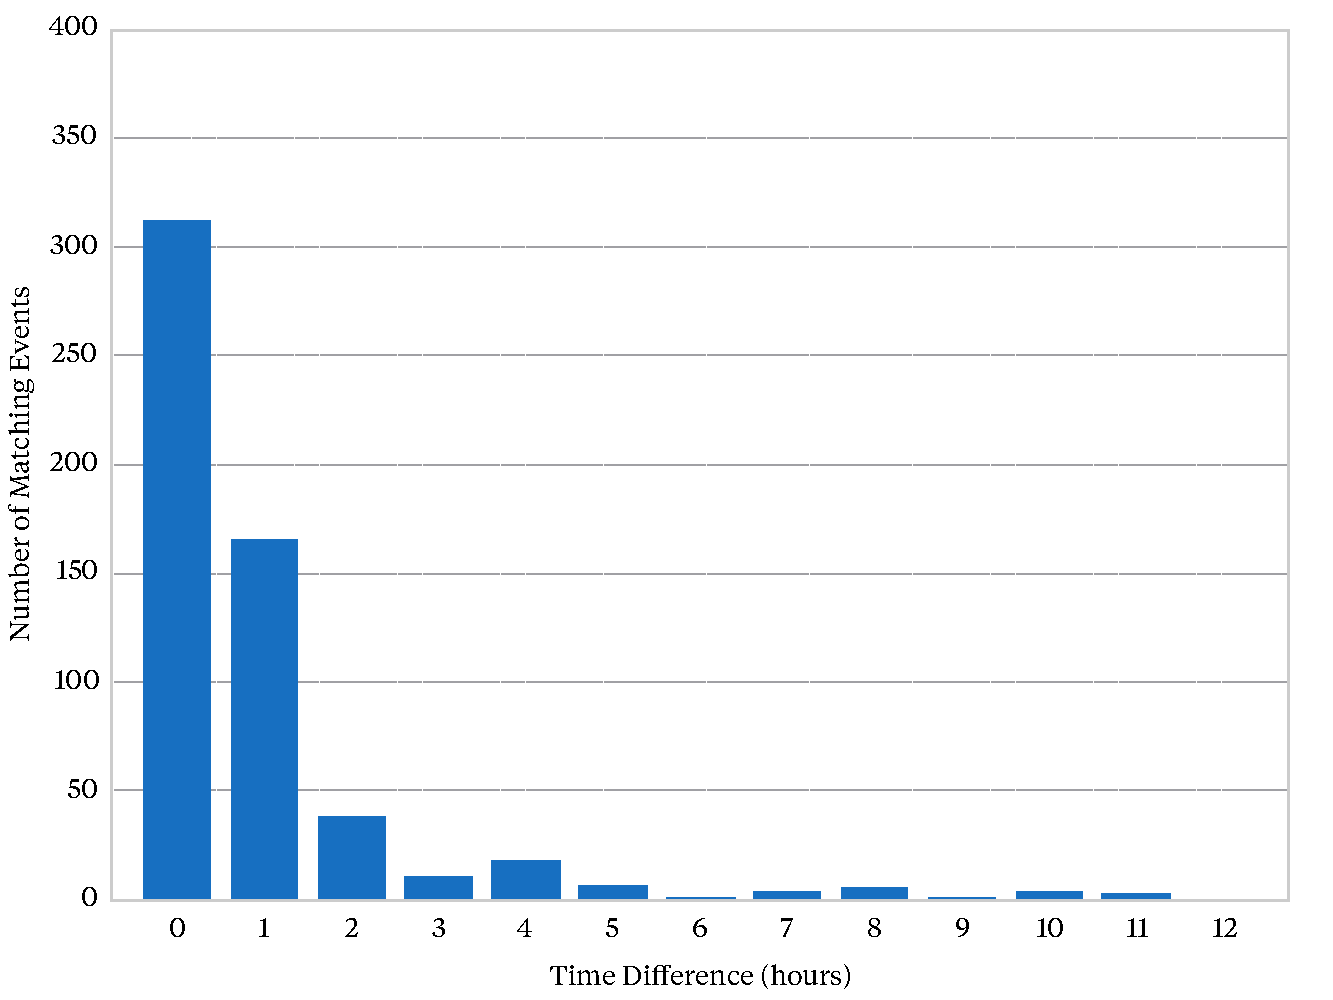
\includegraphics[width=\textwidth]{./Chapters/Collection/images/times}
\caption{The distribution of times between matched events, based upon the number of hours between the centroid times of the events.}
\label{fig:dif_diff}
\end{figure}

It is interesting to note that, although we could have used the number of shared tweets as a feature for clustering, it would have made no difference to resulting clusters.
Out of 41 cases where events share more than 10 tweets, there is only a single case where they do not have a similarity score above our threshold, and the events are subsequently clustered through shared similarity to a 3rd event.
This helps to demonstrate the effectiveness and robustness of our event clustering technique.

\section{Results \& Discussion}
\label{collection:sec:results}
In this section, we describe the results of our evaluation.
We being by describing the characteristics of the generated corpus, and discuss the effectiveness of the different approaches.
We then discuss the annotator agreement, and discuss possible reasons for differences in agreement between the two approaches.

\subsection{Corpus Characteristics}
After clustering, 506 \emph{top-level events} (i.e. events created by combining events from different sources) were produced.
In total, 367 events were clustered to create 77 top-level events, and a further 429 top-level events were created using individual events.

As expected, the detection approach seems to closely reflect to the types of events most commonly discussed on Twitter~\cite{zhao2011empirical}, while the Wikipedia approach gives a more realistic representation of real-world events.
As shown in Table~\ref{table:eventsByCat}, both approaches produced very different distributions of results, however seem to complement each other, and the combined results show much less variation.
For example, the detection approach contributes a large number of \emph{Sports} events, something which is lacking from the Wikipedia approach.
Likewise, the Wikipedia approach contributes a large number of events from \emph{Armed Conflicts and Attacks}, and \emph{Business and Economy}, both categories where the detection approach produces less results.
This could be due to the volume of discussion associated with each of these topics.
\emph{Law, Politics and Scandals} have very few tweets per event in comparison with Sports, meaning that restricting the detection approaches to clusters with at least 30 tweets could have removed many which were discussing these events.
Since we did not put this restriction in place for the Wikipedia approach, it would not have
Table~\ref{table:eventsByCat} shows the events broken down by category and the type of approach used to generate the event.

\begin{table}[h!]
	\centering

	\caption{The distribution of events across the 8 different categories, broken down by method used. The LSH, CS and Wiki columns show numbers of events \emph{before} clustering, while the Clustered column shows the number of events \emph{after} clustering has been performed. }
	\label{table:eventsByCat}

	\begin{tabulary}{\textwidth}{l c c c c}
	\toprule
	\textbf{Category} & \textbf{Clustered} & \textbf{LSH} & \textbf{CS} & \textbf{Wiki}  \\
	\midrule

	Armed Conflicts \& Attacks 			& 98 	& 3 	& 1 	& 95 \\
	Arts, Culture \& Entertainment 		& 53 	& 26 	& 3 	& 34 \\
	Business \& Economy 				& 23 	& 2 	& 1 	& 22 \\
	Disasters \& Accidents 				& 29 	& 16 	& 4 	& 23 \\
	Law, Politics and Scandals 			& 140 	& 124 	& 12 	& 128 \\
	Miscellaneous 						& 21	& 26 	& 6 	& 3 \\
	Science and Technology 				& 16 	& 10 	& 2 	& 11 \\
	Sports 								& 126 	& 175 	& 24 	& 26 \\

	\bottomrule
	\end{tabulary}

\end{table}

The detection method contributed to 186 top-level events, while the Wikipedia approach contributed 342, almost double that of the detection method.
However, the detection approaches contribute over 110,000 of the ~150,000 relevance judgements in the corpus, with an average of 259 tweets per event cluster.
The Wikipedia approach contributes just 39,980 of the relevance judgements, at an average of 85 tweets per event.
This is presumably because of the different types of event identified by each of the methods.
While the detection approaches rely on the volume of tweets to identify events, the Wikipedia approach does not, meaning that it produces a much larger number of smaller events.
The combination of the two approaches allows their different characteristics to complement each other, producing a much more robust corpus than would have been produced had a single approach been used.
If only one approach had been used, then the results would have been unevenly skewed towards either sports or Law and Political discussion, where as the use of both approaches smooths these out to be reflect both the types of event which are happening in the world, as well as what is being discussed on Twitter.

\subsection{Annotator Agreement}
\label{sec:agreement}
The choice of 5 annotators for the evaluation of the detection approach was useful for a number of reasons, as has already been discussed in section~\ref{sec:numAnnotators}, and appears to have been a reasonable choice.
Event agreement increases slightly when 5 annotators are used as opposed to 3 (\(k = 0.91\) and \(k = 0.82\) respectively, using Free-marginal multirater kappa~\citep{Randolph}), whilst agreement at a tweet level remains almost unaffected between 5 and 3 annotators (\(k = 0.91\) and \(k = 0.90\) respectively).
Although this suggests that perhaps 3 annotators would have been sufficient for the evaluation of the detection approaches, it would have resulted in many cases where fewer than 3 annotators judged the tweets for a candidate event, breaking the requirements we outlined in section~\ref{sec:numAnnotators}.

In the case of the Wikipedia approach, tweet agreement was much lower at 0.72, although this still shows very strong agreement between annotators.
It is difficult to say why the agreement is lower for the Wikipedia approach.
However, we hypothesizes that the majority of low quality annotators simply take the easy option for the detection approaches (i.e. answer `no' to the first question), and never actually judge the tweets.
Whereas for the Wikipedia approach, there is no ``easy'' option, so lazy quality annotators have a detrimental effect on the quality of the results.

Annotator agreement was substantial across the TDT categories (\(k = 0.76\)). Agreement was further improved when the combined categories were used, giving near-perfect agreement (0.81).
This shows that our combined categories not only helped to create a category mapping between the different approaches, but also helped to improve agreement, and thus the categorization of events.